% !TEX encoding = UTF-8 Unicode
\documentclass[10pt,usepdftitle=false,aspectratio=169]{beamer}
\usepackage[left]{muibkitsec}
\usepackage{listings}

\usepackage{microtype}
\usepackage{graphbox}
\usepackage{booktabs} 

\usepackage{amsmath,amssymb,amsfonts,amsthm,mathtools}
\usepackage{algorithmic}
\usepackage{textcomp}
\usepackage{xcolor}
\usepackage{diagbox}
\usepackage{float, multirow}
\usepackage{tikz, pgfplots}
\usepackage{tikzsymbols}
\usetikzlibrary{spy}
\usepackage{subcaption}
\usepgfplotslibrary{groupplots}
\pgfplotsset{compat=newest}

% ------------------------------------------------------------------------
\title{Adversarial Label Flips}
\author{Matthias Dellago \& Maximilian Samsinger}
\date{10 June 2021}

% ------------------------------------------------------------------------

\begin{document}
\DeclarePairedDelimiter\abs{\lvert}{\rvert}%
\DeclarePairedDelimiter\norm{\lVert}{\rVert}%
\DeclarePairedDelimiter\ceil{\lceil}{\rceil}
\DeclarePairedDelimiter\floor{\lfloor}{\rfloor}

\begin{frame}[plain]
	\maketitle
\end{frame}	


\begin{frame}[noframenumbering,fragile]
	\frametitle{Fast gradient sign method}
	\begin{tabular}{ccccc}
		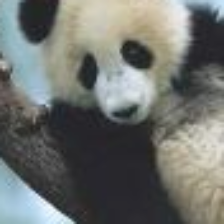
\includegraphics[align=c,width=0.28\columnwidth]{plots/panda_577.png} & \Huge{+} & \Huge{\textbf{$\epsilon$}}\ 
\includegraphics[align=c,width=0.28\columnwidth]{plots/nematode_082.png}\ & \Huge{=} & 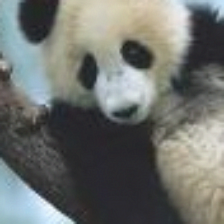
\includegraphics[align=c,width=0.28\columnwidth]{plots/gibbon_993.png} \\~\\
		\huge{Panda} &&\qquad \large{$\operatorname{sign}(\nabla_x\ J(\theta,x,y))$}&& \huge{Gibbon} \\
		(57.7\% confidence) &&&& (99.3\% confidence) 
	\end{tabular}
	\source{[2] Explaining and harnessing adversarial examples, 2014}
\end{frame}

\begin{frame}[fragile]
	\frametitle{What we want to do}
	\begin{block}{Confusion Matrix}
		\begin{table}
			\setlength{\extrarowheight}{2pt}
			\begin{tabular}{cc|c|c|c|}
				& \multicolumn{1}{c}{} & \multicolumn{3}{c}{Categorised as}\\
				& \multicolumn{1}{c}{} & \multicolumn{1}{c}{Dog}  & \multicolumn{1}{c}{Cat} & \multicolumn{1}{c}{Plane} \\\cline{3-5}
				\multirow{3}*{Adversarial Example of a}  & Dog & 0.0 & ? & ?\\\cline{3-5}
				& Cat & ? & 0.0 &  ? \\\cline{3-5}
				& Plane & ? & ? &  0.0 \\\cline{3-5}
			\end{tabular}
		\end{table}
		How many modified dogs get classified as cats vs as planes? etc.
	\end{block}
\end{frame}

\begin{frame}[fragile]
	\frametitle{Quantifying Changes}

	\begin{tabular}{cccc}
		
	$L^0$-Norm & 	$L^1$-Norm & 	$L^2$-Norm & 	$L^\infty$-Norm \vspace{5pt} \\
	
	
	
	\shortstack{Number of \\ pixels changed} & \shortstack{Sum of \\ all changes} & \shortstack{Sum of the $square$ \\ of all changes} & \shortstack{Maximum of \\ all changes} \\
	
	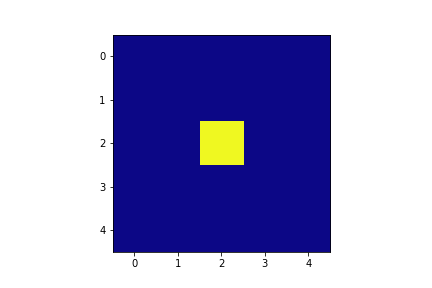
\includegraphics[align=c,width=0.3\columnwidth]{plots/L0.png} &
	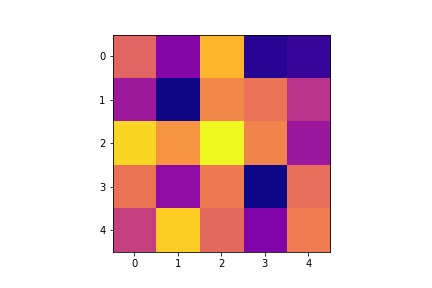
\includegraphics[align=c,width=0.3\columnwidth]{plots/L1.png} &
	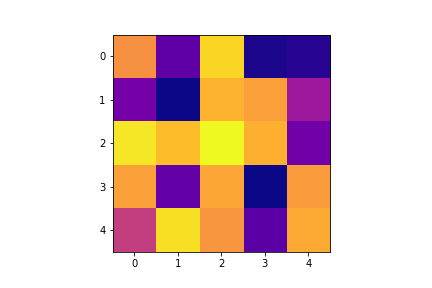
\includegraphics[align=c,width=0.3\columnwidth]{plots/L2.png} &
	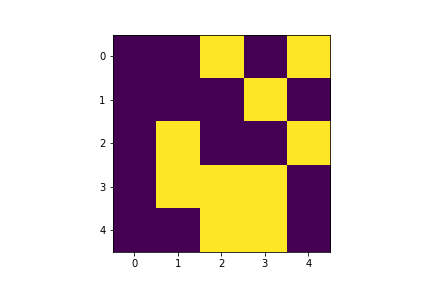
\includegraphics[align=c,width=0.3\columnwidth]{plots/Linf.png} &
	
	\end{tabular}
\end{frame}

\begin{frame}[allowframebreaks]
	\frametitle{References}
	\bibliographystyle{unsrt}
	\bibliography{literature}
\end{frame}


\end{document}
